\newpage
\section{Tests du logiciel}

\subsection{Tests unitaires}

\paragraph{}
Les tests, absents de la version du logiciel VisualImpro livrée par
Jérémy Lixandre, ont été entièrement implémentés par nos soins. Nous
les avons regroupés dans un dossier \verb!Tests! qui comprend un
fichier source \verb!TestMain.cpp!, lequel affiche les résultats de
tous les autres fichiers de test sur la sortie standard, et six
répertoires contenant ces fichiers de test. Il contient également un
\verb!Makefile! et un répertoire \verb!Sine-samples! contenant des
signaux sinusoïdaux à tester.

\subsubsection{Tests de classes}
\paragraph{}
Le répertoire \verb!TestClasses! vérifie le bon fonctionnement de
certaines classes.

\paragraph{}
Le fichier \verb!TestMatrix.cpp! est implémenté dans le but de
démontrer le correct fonctionnement de la classe codant l'objet
matrice, de la classe \verb!Matrix.cpp!. Il teste des opérations
portant sur des matrices, sur des cases, des lignes et des colonnes
spécifiques de matrices.

\paragraph{}
Le fichier \verb!TestMultiCorrel.cpp! teste des opérations de base sur
l'objet permettant de traiter le retour sonore,
\verb!ProcessMultiCorrel.cpp!, telles que des opérations d'accès et
d'écriture basiques \textit{getter/setter} aux données membres de la
classe.

\subsubsection{Tests de la fonction de traduction du coefficient de corrélation en triplets RGB}
\paragraph{}
Le répertoire \verb!TestColor! contient deux fichiers de test testant
chacun le bon fonctionnement des deux fonctions de traduction du
coefficient de corrélation en triplet RGB (la première établit un code
couleur allant du rouge au vert, la seconde un code couleur en niveaux
de gris allant du noir au blanc). Ces tests fonctionnent en vérifiant
que des flottants ayant des valeurs extrêmes et une valeur
intermédiaire retournent bien les couleurs attendues, par exemple :
une couleur rouge pour un coefficient de 0 avec la première fonction.

\subsubsection{Tests de la fonction de pré-traitement}
\paragraph{}
Le répertoire \verb!TestPreproc! contient trois fichiers de test, un
pour chacune des trois fonctions de pré-traitement
existantes. L'implémentation de \verb!TestPreprocDefault.cpp!,
\verb!TestPreprocEnergy.cpp! et \verb!TestPreprocStrenghtEnergy.cpp!
permet de comparer le résultat des fonctions de pré-traitement
correspondantes, prenant des matrices simples en paramètres, avec les
résultats attendus.

\subsubsection{Tests de la fonction de calcul de coefficient de corrélation}
\paragraph{}
Le répertoire \verb!TestCoeff! contient deux fichiers testant chacun
l'une de nos deux fonctions de calcul de coefficient de
corrélation. Le premier, \verb!TestCoeffScalar.cpp!, vérifie que la
fonction testée renvoie bien la bonne valeur en comparant son résultat
pour deux vecteurs arbitraires passés en paramètre avec le résutat du
calcul brut du produit scalaire de ces deux mêmes vecteurs, qui
doivent être égaux. Le second fichier de test unitaire,
\verb!TestCoeffRandom!, teste que pour mille itérations, le résultat
de la fonction testée est toujours compris dans l'ensemble de valeur
attendu (entre 0 et 1).

\subsubsection{Tests de la fonction de mixage}
\paragraph{}
Les fichiers contenus dans le répertoire \verb!TestMix! s'assurent
pour chaque fonction de mixage existante que le résultat obtenu pour
une matrice passée en paramètre de la fonction est égal à celui
attendu. Par exemple, la fonction de \verb!MixNeutral.cpp!, qui simule
l'absence de fonction de mixage, doit renvoyer 1 comme coefficient de
modification du volume sonore quelque soit la matrice d'entrée ; on
s'en assure dans le fichier de test \verb!TestMixNeutral.cpp!.

\subsubsection{Test de l'interface graphique utilisateur}
Les fichiers contenus dans le répertoire \verb!TestGUI! assurent
le fonctionnement de l'interface graphique. Le seul test implémenté
et le test du builder qui est la seule classe qui construit le fichier description
de configuration.
En effet, hormis en utilisant une capture d'écran de l'affichage voulu afin
de la comparer à celle qui est affichée, il est difficile de tester
une interface graphique.

\subsection{Test globaux}
\paragraph{}
Pour tester l'outil dans son intégralité, i lfallait des échantillons pour lesquels nous connaissions les résultats à l'avance. Pour cela, nous avons généré des signaux sinusoïdaux et carrés, car ce sont les signaux les plus simples. Nous en avons généré plusieurs, et à chaque fois, nous avons décalé les phases pour pouvoir réaliser plusieurs tests. De plus, nous avons réalisé nos tests avec deux focntions de pré-traitement différentes : \verb!PreprocDefault! et \verb!PreprocStrengthEnergy!. La première ne touche pas au signal, la seconde transforme la composante négative en positive.
\subsubsection{Avec PreprocDefault}
\paragraph{}
Les figures suivantes doivent être interprétées de la façon suivante : plus la couleur est verte, plus les signaux sont proches, plus on tend vers le rouge, plus les signaux sont différents.
\begin{figure}[H]
    \centering
    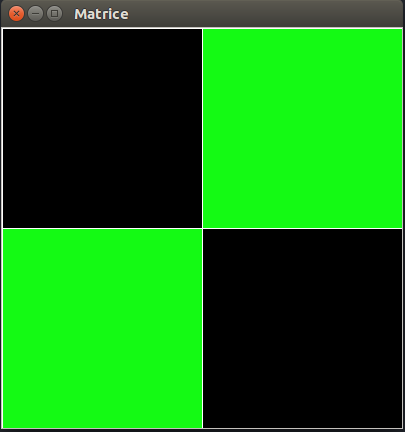
\includegraphics[scale=0.3]{assets/Captures-sinus/PreprocDefaultnormal-normal.png}
    \caption{Test avec deux sinus identiques}
    \label{}
\end{figure}
\begin{figure}[H]
    \centering
    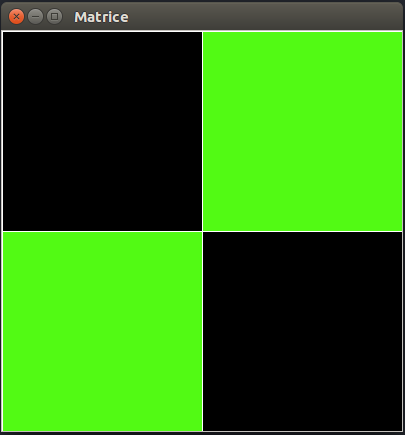
\includegraphics[scale=0.3]{assets/Captures-sinus/PreprocDefaultnormal-30.png}
    \caption{Test avec deux sinus décalés de 30 degrés}
    \label{}
\end{figure}
\begin{figure}[H]
    \centering
    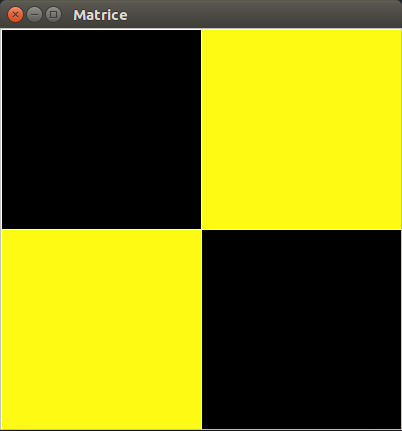
\includegraphics[scale=0.3]{assets/Captures-sinus/PreprocDefaultnormal-60.png}
    \caption{Test avec deux sinus décalés de 60 degrés}
    \label{}
\end{figure}
\begin{figure}[H]
    \centering
    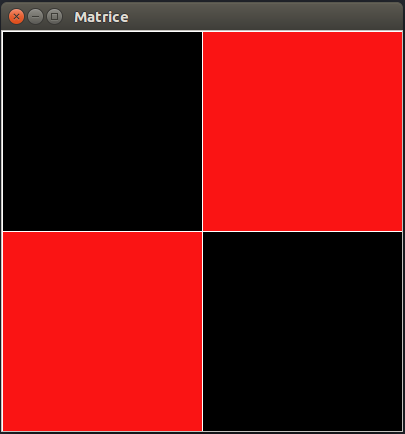
\includegraphics[scale=0.3]{assets/Captures-sinus/PreprocDefaultnormal-90.png}
    \caption{Test avec deux sinus décalés de 90 degrés}
    \label{}
\end{figure}
\paragraph{}
À 90 degrés, les sinus sont inversées, d'où le fait que la corrélation soit nulle.
\begin{figure}[H]
    \centering
    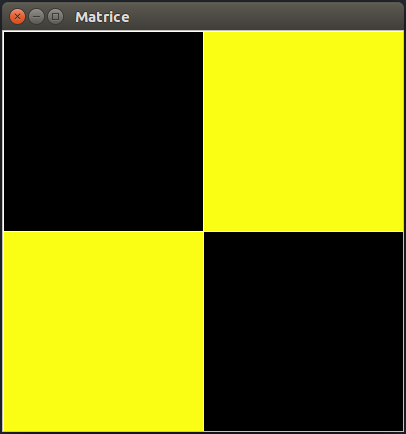
\includegraphics[scale=0.3]{assets/Captures-sinus/PreprocDefaultnormal-120.png}
    \caption{Test avec deux sinus décalés de 120 degrés}
    \label{}
\end{figure}
\begin{figure}[H]
    \centering
    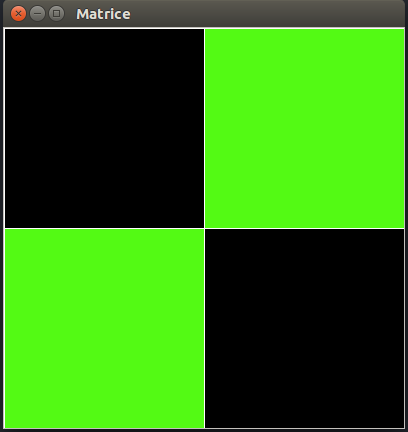
\includegraphics[scale=0.3]{assets/Captures-sinus/PreprocDefaultnormal-150.png}
    \caption{Test avec deux sinus décalés de 150 degrés}
    \label{}
\end{figure}
\begin{figure}[H]
    \centering
    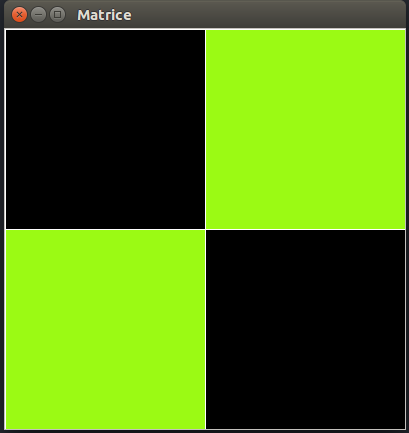
\includegraphics[scale=0.3]{assets/Captures-sinus/PreprocDefautnormal-180.png}
    \caption{Test avec deux sinus décalés de 180 degrés}
    \label{}
\end{figure}
\subsubsection{Avec PreprocStrenghtEnergy}
\begin{figure}[H]
    \centering
    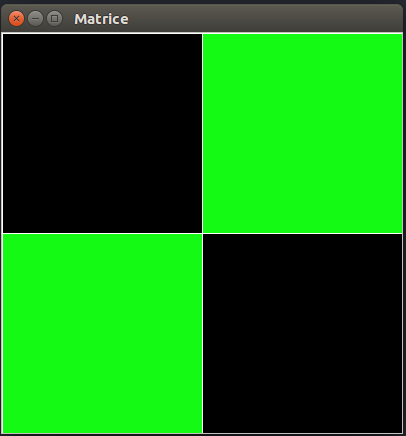
\includegraphics[scale=0.3]{assets/Captures-sinus/PreprocStrengthnormal-normal.png}
    \caption{Test avec deux sinus identiques}
    \label{}
\end{figure}
\begin{figure}[H]
    \centering
    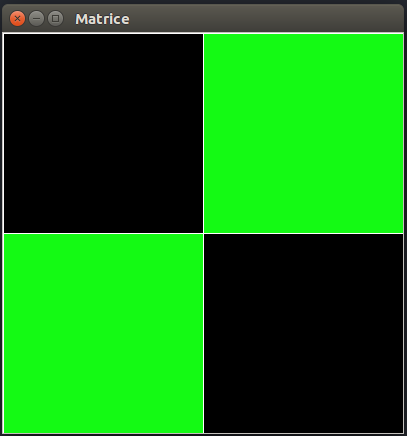
\includegraphics[scale=0.3]{assets/Captures-sinus/PreprocStrengthnormal-90.png}
    \caption{Test avec deux sinus décalés de 90 degrés}
    \label{}
\end{figure}
\paragraph{}
Avec PreprocStrenghtEnergy, comme il n'y a plus de valeurs négatives, la sinus décalée de 90 degrés est identique à la sinus normale.
\begin{figure}[H]
    \centering
    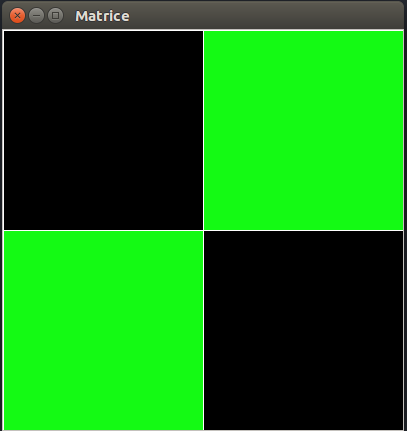
\includegraphics[scale=0.3]{assets/Captures-sinus/PreprocStrenghtnormal-180.png}
    \caption{Test avec deux sinus décalés de 180 degrés}
    \label{}
\end{figure}